\documentclass{amsart}[11pt,fullpage]

%\usepackage[all]{xy}
\usepackage{amsmath,amssymb,amsthm}
\usepackage{tikz}

\usetikzlibrary{decorations.pathreplacing,decorations.markings}


\usepackage{xcolor}
\def\todoit{{\color{red} $^{TODO}$}} %!!!!!!!!!!!!!!!!!!!! I CHANGED YOUR COMMAND. !!!!!!!!!!!!!!!!!!!!
%%%%%%%%%%%%%%%%%%%%%%%%%%%%%%%%%%%%%%%%%%%%%%%%%%%%%%%%%%%%%%%%%%%%%%%%%%%%%%%%%%%%%%%%%%%%%%%%%%%%%%%
%I'm trying an alternate todo note setup that will give us a quick glance at start of document of those things that need doing. The relevant package is on the next line, and the List of Todos setup is right before the \begin{document} command.
%%%%%%%%%%%%%%%%%%%%%%%%%%%%%%%%%%%%%%%%%%%%%%%%%%%%%%%%%%%%%%%%%%%%%%%%%%%%%%%%%%%%%%%%%%%%%%%%%%%%%%%
\def\ltblue{blue!20!white}
\def\ltgreen{green!20!white}

\usepackage[colorinlistoftodos, textsize=tiny]{todonotes}

%\headheight 35pt
%
%\setlength{\textwidth}{6.5in}      %%%%%%%%%%%%%%%%%%%%%%%%%%%%%%%%%%%%%%%%%%%%%%%%%%%%%%%%%%%%%%%%%%%
%\setlength{\oddsidemargin}{0in}    Is it OK if we undo these formatting commands?
%\setlength{\evensidemargin}{0in}   %%%%%%%%%%%%%%%%%%%%%%%%%%%%%%%%%%%%%%%%%%%%%%%%%%%%%%%%%%%%%%%%%%%
%\setlength{\textheight}{8.5in}
%\setlength{\topmargin}{0in}
%\setlength{\headheight}{0in}
%\setlength{\headsep}{12pt}
%\setlength{\footskip}{.5in}

\renewcommand{\theenumi}{\roman{enumi}}

\tikzset{
  % style to apply some styles to each segment of a path
  on each segment/.style={
    decorate,
    decoration={
      show path construction,
      moveto code={},
      lineto code={
        \path [#1]
        (\tikzinputsegmentfirst) -- (\tikzinputsegmentlast);
      },
      curveto code={
        \path [#1] (\tikzinputsegmentfirst)
        .. controls
        (\tikzinputsegmentsupporta) and (\tikzinputsegmentsupportb)
        ..
        (\tikzinputsegmentlast);
      },
      closepath code={
        \path [#1]
        (\tikzinputsegmentfirst) -- (\tikzinputsegmentlast);
      },
    },
  },
  % style to add an arrow in the middle of a path
  mid arrow/.style={postaction={decorate,decoration={
        markings,
        mark=at position .5 with {\arrow[#1]{stealth}}
      }}},
}


\newcommand{\oarc}[4]{
\draw[thick, postaction={on each segment={mid arrow}}] (#1,#2) ..controls (#1 + .2,#2 + .7) and (#3 - .2,#4 + .7) .. (#3,#4);
}



\def\l{{\left(}}
\def\r{{\right)}}

\def\Z{{\mathbb Z}}
\def\C{{\mathbb C}}
\def\R{{\mathbb R}}
\def\D{{\mathbb D}}
\def\H{{\mathbb H}}
\def\P{{\mathbb P}}

\def\F{{\mathcal F}}
\def\M{{\mathcal M}}
\def\O{{\mathcal O}}
\def\A{{\mathcal A}}
\def\cl{\mathcal}

\def\s{{\sigma}}
\def\t{{\tau}}
\def\k{{\kappa}}

\def\g{\gamma}
\def\a{\alpha}
\def\xibar{\bar{\xi}}

\def\Xtilde{\widetilde{X}}
\def\etilde{\tilde{e}}

\def\bs{\backslash}
\def\dot{\bullet}

\def\G{{\Gamma}}
\def\SL{\mathrm{SL}}
\def\GL{\mathrm{GL}}
\def\O{\mathrm{O}}
\def\SO{\mathrm{SO}}
\def\U{\mathrm{U}}
\def\SU{\mathrm{SU}}
\def\PSL{\mathrm{PSL}}

\def\Gtilde{\widetilde{G}}
\def\SLtilde{\widetilde{\SL}}

\def\ar{\operatorname{ar}}
\def\mr{\operatorname{mr}}


\def\sing{{\mathrm{sing}}}

\newcommand\id{\operatorname{id}}
\newcommand\inter{\operatorname{int}}
\newcommand\Aut{\operatorname{Aut}}
\newcommand\Gal{\operatorname{Gal}}
\newcommand\rel{\operatorname{rel}}
\newcommand\Tr{\operatorname{Tr}}
\newcommand\End{\operatorname{End}}
\newcommand\diag{\operatorname{diag}}
\newcommand\perm{\operatorname{perm}}
\newcommand\Sp{\Sigma^{(p)}}
\newcommand\SpPm{\Sigma^{\pm(p)}}
\newcommand\SpM{\Sigma^{-(p)}}

\newtheorem{thm}{Theorem}[section]
\newtheorem{lem}[thm]{Lemma}
\newtheorem{prop}[thm]{Proposition}
\newtheorem{cor}[thm]{Corollary}

\theoremstyle{definition}
\newtheorem{defn}[thm]{Definition}
\newtheorem{rem}[thm]{Remark}

%\newenvironment{definition}[1][Definition]{\begin{trivlist}
%\item[\hskip \labelsep {\bfseries #1}]}{\end{trivlist}}
%\newenvironment{ex}[1][Example]{\begin{trivlist}
%\item[\hskip \labelsep {\bfseries #1}]}{\end{trivlist}}
%\newenvironment{rem}[1][Remark]{\begin{trivlist}
%\item[\hskip \labelsep {\bfseries #1}]}{\end{trivlist}}

\makeatletter
\providecommand\@dotsep{5}
\def\listtodoname{List of Todos}
\def\listoftodos{\@starttoc{tdo}\listtodoname}
\makeatother

\begin{document}

\listoftodos
%%%%%%%%%%%%%%%%%%%%%%%%%%%%%%%%%%%%%%%%%%%%%%%%%%%%%%%%%%%%%%%%%%%%%%%%%%%%%%%%%%%%%%%%%%%%%%%%%%%%%%%%%
% BLUE is for David
% GREEN is for Cornwell
%%%%%%%%%%%%%%%%%%%%%%%%%%%%%%%%%%%%%%%%%%%%%%%%%%%%%%%%%%%%%%%%%%%%%%%%%%%%%%%%%%%%%%%%%%%%%%%%%%%%%%%%%
\newpage




%\title{The Augmentation Rank of Knot Cables}
%\author{David Hemminger\footnote{The author would like to thank Dr.\ Christopher Cornwell for the advising, and everyone else for the patience.}\\ Duke University}
%\maketitle

\title{Augmentation Rank of Satellites with Braid Pattern}

\author{David R. Hemminger}
\author{Christopher R. Cornwell}

\begin{abstract}
Given a knot $K$ in $S^3$, a question raised by Cappell and Shaneson asks if the meridional rank of $K$ equals the bridge number of $K$. Using augmentations in knot contact homology we consider the persistence of equality between these two invariants under satellite operations on $K$ with a braid pattern. In particular, we answer the question in the affirmative for a large class of iterated torus knots.
\end{abstract}

\maketitle

\section{Introduction}
Let $K$ be an oriented knot in $S^3$ and denote by $\pi_K$ the fundamental group of the knot complement $\overline{S^3\setminus n(K)}$. We call an element of $\pi_K$ a \emph{meridian} if it is represented by the oriented boundary of a disc $D$ embedded in $S^3$ such that $D$ intersects $K$ geometrically once on its interior. The group $\pi_K$ is generated by meridians; the \emph{meridional rank} of $K$, written $\mr(K)$, is the minimal size of a generating set containing only meridians. 

Choose a height function $h:S^3\to\R$. The \emph{bridge number} of $K$, denoted $b(K)$, is the minimal number of local maxima of $h|_{K}$ among all realizations of $K$. Equivalently, call a 2-sphere $S\subset S^3$ a bridge sphere if each ball in $S^3\setminus S$ intersects $K$ in some number $b(S,K)$ of trivial arcs. The minimum of $b(S,K)$ over all bridge spheres and all realizations of $K$ equals $b(K)$.

A basic argument shows that $\mr(K)\le b(K)$ for any $K\subset S^3$. Whether this bound is, in fact, equality for all knots is an open question asked by Cappell and Shaneson \cite[Prob. 1.11]{Kir95}. Equality is known to hold for some families of knots due to work of various authors. 

In this paper we study the behavior of augmentations, which arise in the study of knot contact homology, upon taking satellites of $K$ with a braid pattern. As we explain below, augmentations provide a lower bound on $\mr(K)$ which is sometimes large enough to force $\mr(K)=b(K)$. Our main result shows that for many braid patterns this equality will persist upon taking a satellite if augmentations forced the equality for $K$.

More precisely, suppose that $B\in B_k$ and $B'\in B_p$ are two braids (here $B_n$ denotes Artin's group of $n$-braids) and that $K$ is the braid closure of $B$ (see Figure \ref{fig:BClosure} below). Denote by $B^{(p)}$ the braid in $B_{kp}$ which consists of each strand of $B$ being replaced by $p$ parallel copies of that strand (in the blackboard framing). Also, include $B'$ into $B_{kp}$ by coupling it with an identity braid on $(k-1)p$ strands. The \emph{braid satellite} of $K$ associated to $B, B'$ is the braid closure of $B^{(p)}B'$, denoted $K(B,B')$.

Augmentations of $K$ have an associated \emph{rank}, and we write $\ar(K)$ for the maximum rank among all augmentations of $K$. This number is well-defined and we have the following inequalities (see Section \ref{SecBG_AugRk})
      \begin{equation}
      \ar(K)\le\mr(K)\le b(K)
      \label{Eqn:ARvMRvb}
      \end{equation}

To minimize notation, we will write $\ar(B)$ to denote the augmentation rank of the braid closure of a braid $B$. We show the following. 

\begin{thm}\label{main}
If $B$ is a $k$-braid such that $\ar(B)=k$ and $B'$ a $p$-braid such that $\ar(B')=p$ then $\ar(K(B,B'))=kp$.
\end{thm}

\begin{rem}Our theorem shows that if $B, B'$ have largest possible augmentation rank (equal to their index) then the augmentation rank acts multiplicatively under braid satellites. It is natural to ask if this multiplicative property holds under weaker assumptions on $B, B'$. Braid stabilization provides a way to construct counterexamples to augmentation rank being multiplicative, even when the bridge number does multiply.
\label{rem:BrSatNotMult}
\end{rem}

A corollary to Theorem \ref{main} involves Cappell and Shaneson's question for iterated torus knots. Let ${\bf p}=(p_1,\ldots,p_n)$ and ${\bf q}=(q_1,\ldots,q_n)$ be integral vectors. We write $T({\bf p},{\bf q})$ for the $({\bf p},{\bf q})$ \emph{iterated torus knot}, defined as follows. Define $T({\bf p},{\bf q})$ inductively so that, if $\widehat{\bf p}, \widehat{\bf q}$ are the truncated lists obtained from ${\bf p},{\bf q}$ by removing the last integer in each, then $T({\bf p},{\bf q})$ is the $(p_n,q_n)$-cable of $T(\widehat{\bf p},\widehat{\bf q})$. By convention $T(\emptyset,\emptyset)$ is the unknot.

The knot (or link) $T({\bf p},{\bf q})$ is only well-defined if a framing convention is chosen at each stage of cabling. The traditional choice is to take the Seifert framing at each stage. In the statement of the corollary below, we use a different convention which is suited to the braid satellite construction (see Section \ref{SecMainCor}).

\begin{cor}\label{cor:iteratedCables}
Given integral vectors ${\bf p}$ and ${\bf q}$, suppose that $|p_i|<|q_i|$ and $\text{gcd}(p_i,q_i)=1$ for each $1\le i\le n$. Then $\ar(T({\bf p},{\bf q}))=p_1p_2\ldots p_n$. Moreover, $\mr(T({\bf p},{\bf q})) = b(T({\bf p},{\bf q}))$ for all such ${\bf p}$ and ${\bf q}$.
\end{cor}


%Let $\tau_{m,l} \in B_{pk}$ be defined by $\tau_{m,l} = \s_m\s_{m+1}\cdots\s_{m+l-1}$, and let $\Sp_n\in B_{pk}$ be defined by $\Sp_n = \tau_{np,p}\tau_{np-1,p}\cdots\tau_{np-p+1,p}$ (see Figure \ref{FigSigma2}). Then if $B\in B_k$ is given by the braid word $\s_{n_1}\s_{n_2}\cdots\s_{n_m}$, we define the \emph{$p$-copy} $B^{(p)}$ of $B$ to be $B^{(p)} = \Sp_{n_1}\Sp_{n_2}\cdots\Sp_{n_m}$. Our main result shows that certain satellites with a braid pattern of knots with augmentation rank equal to braid index also have augmentation rank equal to bridge index.

%FigSigma2
%\begin{figure}[ht]
%\begin{tikzpicture}[xscale=0.5,yscale=0.4,>=stealth]
%\draw(0,2)--(4,4);
%\draw(0,3)--(4,5);
%\draw[very thick,draw=white,double=black](0,4)--(4,2);
%\draw[very thick,draw=white,double=black](0,5)--(4,3);
%\draw(0,0)--(4,0);
%\draw(0,1)--(4,1);
%\draw(2.5,-1) node {$\Sigma_1$};
%\end{tikzpicture}
%\caption{$\Sigma^{(2)}_1$}
%\label{FigSigma2}
%\end{figure}


The paper is organized as follows. In Section \ref{SecBG} we give the needed background in knot contact homology and discuss the rank of augmentations and the relationship to the meridional rank. In Section \ref{SecBG_AugExist} we review some techniques that will be used in the proof of Theorem \ref{main}. We also discuss there the difficulty of generalizing Theorem \ref{main} to braid satellites of knots with smaller augmentation rank. Section \ref{SecMain} is mainly devoted to the proof of Theorem \ref{main}.



%\begin{cor}\label{cor:cables}
%Let $K$ be a knot with augmentation rank equal to its braid index, and let $p,q>0$ with $\gcd(p,q) = 1$ and $p<q$. Then the $(p,q)$-cable of $K$ taken with the blackboard framing has augmentation rank equal to its braid index.
%\end{cor}




%\newtheorem*{thm:RanknAugs}{Theorem \ref{thm:RanknAugs}}
%  \begin{thm:RanknAugs}[\cite{Cor13a}] If $K$ is the closure of $B\in B_n$ and has a rank $n$ augmentation $\epsilon:\A_n\otimes R_0\to\C$, then 
%    \begin{equation*}\tag{\ref{eqn:FindingAugs}}
%    \epsilon(\Phi_B^L)=\Delta(B)=\epsilon(\Phi_B^R).
%    \end{equation*}
%    Furthermore, any homomorphism $\epsilon:\A_n\to\C$ which satisfies (\ref{eqn:FindingAugs}) can be extended to $\A_n\otimes R_0$ to produce a rank $n$ augmentation of $K$. 
%  \end{thm:RanknAugs}






%Define ar
%generated by entries of $A_{ij}$





\section{Background}
\label{SecBG}

  We review in Section \ref{SecBG_KCHdef} the construction of $HC_0(K)$ from the viewpoint of the combinatorial knot DGA, which was first defined in \cite{Ng08}; our conventions are those given in \cite{Ng12}. In Section \ref{SecBG_AugRk} we discuss augmentations in knot contact homology and their rank, which gives a lower bound on the meridional rank of the knot group useful for studying the relation between meridional rank and bridge number. Finally, in Section \ref{SecBG_AugExist} is a discussion of techniques from \cite{Cor13a} that we use to calculate the augmentation rank.

  Throughout the paper we denote by $B_n$ the group of $n$-braids. We orient $n$-braids from left to right, labeling the strands $1,\ldots, n$, with 1 the topmost and $n$ the bottommost strand. We work with Artin's generators $\{\sigma_i^{\pm}$, $i=1,\ldots,n-1\}$ of $B_n$, where in $\s_i$ only the $i$ and $i+1$ strands interact, and they cross once in the manner depicted in Figure \ref{fig:BraidGens}.
      \begin{figure}[ht]
        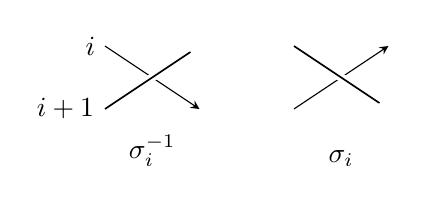
\begin{tikzpicture}[scale=0.4,>=stealth]
        \draw[->] (0,2) -- node[at start,left]{$i$} (3,0);
        \draw[draw=white,very thick,double=black,->] (0,0) -- node[at start,left]{$i+1$} (3,2);
        \draw (1.5,-0.5) node[below] {$\sigma_i^{-1}$};

        \draw[->] (6,0) -- (9,2);
        \draw[draw=white,very thick,double=black,->] (6,2) -- (9,0);
        \draw (7.5,-1) node[below] {$\sigma_i$};
        \end{tikzpicture}
        \caption{Generators of $B_n$}
        \label{fig:BraidGens}
      \end{figure}
    Given a braid $B$ the braid closure $\widehat{B}$ of $B$ is the link obtained as shown in Figure \ref{fig:BClosure}. The \emph{writhe} (or algebraic sum) of $B$, denoted $\omega(B)$, is the sum of the exponents in a factorization of $B$ as a product of the $\s_i, i=1,\ldots,n-1$.

    \begin{figure}[ht]
      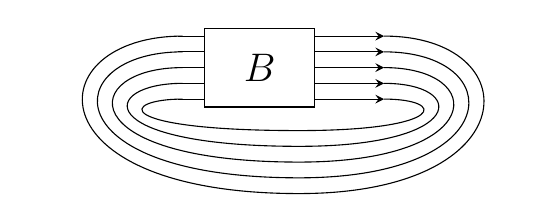
\begin{tikzpicture}[scale=0.4,>=stealth]
      %  \clip (-.7,-1.25) rectangle (7.3,2.5);
        \draw(0,-.25)--(0,2.25)--(3.5,2.25)--(3.5,-.25)--cycle;
        \draw(1.75,1) node {{\Large $B$}};
        \foreach \y in {0,.5,1,1.5,2}
      %    \filldraw (4.75,\y) circle (2pt);
        \foreach \y in {0,.5,1,1.5,2}
          \draw(-.85,\y) -- (0,\y);
        \foreach \y in {0,.5,1,1.5,2} 
          \draw[thin] (3.5,\y) -- (5.25,\y);
        \foreach \y in {0,.5,1,1.5,2} 
          \draw[->] (5.18,\y) -- (5.7,\y);
        \foreach \y in {0,.5,1,1.5,2}
          \draw (5.7,\y) ..controls (7.7+\y*1.3,\y) and (7.7+\y*1.3,-\y-1) ..(3,-\y-1)
                  ..controls (-3-\y*1.3,-\y-1) and (-2.7-\y*1.3,\y)..(-.7,\y);
      %  \draw[red,->]
      %      (4.75,.5) ..controls (5.05,.75) and (5.05,1.25) ..(4.75,1.5);
      %  \draw[draw=white,double=black,very thick]
      %      (4.45,2.1)  ..controls (4.5,2.35) and (4.6,2.5) .. (4.8,2.5)
      %            ..controls (5,2.5) and (5.2,2) .. (5.2 ,1)
      %            ..controls (5.2,0) and (5,-.5) .. (4.8,-.5)
      %            ..controls (4.6,-.5) and (4.5,-.35)..(4.45,-.1);
      %  \draw   (4,-.6) node {{\footnotesize $D$}};
      %  \draw (6.15,1.95) node {{\large $\ast$}};
      %  \draw (-.65,.5) node {{\footnotesize $i$}}
      %      (-.65,1.5) node{{\footnotesize $j$}};
      \end{tikzpicture}
      \caption{The braid closure of $B$}
      \label{fig:BClosure}
    \end{figure}

\subsection{Knot contact homology}
\label{SecBG_KCHdef}

  We review the construction of the combinatorial knot DGA of Ng (in fact, we discuss only the degree zero part as this will suffice for our purposes). This DGA was defined in order to be a calculation of knot contact homology and was shown to be so in \cite{EENS12} (see \cite{Ng12} for more details). Let $\A_n$ be the noncommutative unital algebra over $\Z$ freely generated by $a_{ij}$, $1\le i\ne j\le n$. We define a homomorphism $\phi : B_n \rightarrow\Aut \A_n$ by defining it on the generators of $B_n$:

  \begin{equation}
  \phi_{\s_k}\colon
  \left\{
       \begin{array}{lr}
         a_{ij}\mapsto a_{ij} & i,j\ne k,k+1\\
         a_{k+1,i}\mapsto a_{ki} & i\ne k,k+1\\
         a_{i,k+1}\mapsto a_{ik} & i\ne k,k+1\\
         a_{k,k+1}\mapsto -a_{k+1,k} & \\
         a_{k+1,k}\mapsto -a_{k,k+1} & \\
         a_{ki}\mapsto a_{k+1,i} - a_{k+1,k}a_{ki} & i\ne k,k+1\\
         a_{ik}\mapsto a_{i,k+1} - a_{ik}a_{k,k+1} & i\ne k,k+1\\
       \end{array}
  \right.
  \label{DefnPhiMap}
  \end{equation}

  Let $\iota\colon B_n \rightarrow B_{n+1}$ be the inclusion $\s_i\mapsto\s_i$ so that the $(n+1)$ strand does not interact with those from $B\in B_n$, and define $\phi_B^*\in \Aut \A_{n+1}$ by $\phi_B^* = \phi_B\circ\iota$. We then define the $n\times n$ matrices $\Phi_B^L$ and $\Phi_B^R$ with entries in $\A_n$ by

  $$\phi_B^*(a_{i,n+1}) = \sum_{j=1}^n(\Phi_B^L)_{ij}a_{j,n+1}$$

  $$\phi_B^*(a_{n+1,i}) = \sum_{j=1}^na_{n+1,j}(\Phi_B^R)_{ji}$$

  Finally, let $R_0$ be the Laurent polynomial ring $\Z[\lambda^{\pm1},\mu^{\pm1}]$ and define matrices $\bf{A}$ and $\bf{\Lambda}$ over $R_0$ by

  \begin{equation}
  {\bf A}_{ij} = 
  \left\{
       \begin{array}{lr}
        a_{ij} & i<j\\
        -\mu a_{ij} & i>j\\
        1-\mu & i = j\\
       \end{array}
  \right.
  \label{def:Amatrix}
  \end{equation}
  \begin{equation}
  {\bf \Lambda} = \diag[\lambda\mu^{\omega(B)},1,\ldots,1].
  \label{defn:Lambda}
  \end{equation}

  \begin{defn}
  Suppose that $K$ is the closure of $B\in B_n$. Define $\mathcal{I}\subset \A_n\otimes R_0$ to be the ideal generated by the entries of $\bf{A} - \Lambda\cdot\Phi_B^L\cdot \bf{A}$ and $\bf{A} - \bf{A}\cdot\Phi_B^R\cdot\Lambda^{-1}$. The \emph{degree zero homology of the combinatorial knot DGA} is $\operatorname{HC}_0(K) = (\A_n\otimes R_0)/\mathcal{I}$.
  \label{defn:HC_0}
  \end{defn}
  
  It was shown in \cite{Ng08} that the isomorphism class of $HC_0(K)$ is unchanged by the Markov moves on $B$, hence $HC_0(K)$ is an invariant of the knot $K$. We only consider $HC_0(K)$ here, but there is a larger invariant, the differential graded algebra discussed in \cite{Ng12}.

  The proofs in Section \ref{SecMain} require a number of computations of $\phi_B$ for particular braids $B$. Such computations are greatly benefited by an alternate description of the map $\phi_B$, which we now give and will use without comment in Section \ref{SecMain}.

  Let $D$ be a flat disk, to the right of $B$, with $n$ points (punctures) where it intersects $K=\widehat{B}$ (see Figure \ref{FigA_nGens}). We assume the $n$ punctures of $D$ to be collinear, on a line that separates $D$ into upper and lower half-disks. Denote by $c_{ij}$ the isotopy class (fixing endpoints) of a path that is contained in the upper half-disk of $D$, with initial endpoint on the $i^{th}$ strand and terminal endpoint on the $j^{th}$ strand.

  \begin{figure}[ht]
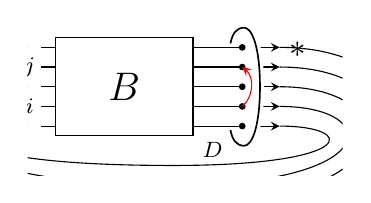
\begin{tikzpicture}[scale=0.5,>=stealth]
  \clip (-.7,-1.25) rectangle (7.3,2.5);
  \draw(0,-.25)--(0,2.25)--(3.5,2.25)--(3.5,-.25)--cycle;
  \draw(1.75,1) node {{\Large $B$}};
  \foreach \y in {0,.5,1,1.5,2}
    \filldraw (4.75,\y) circle (2pt);
  \foreach \y in {0,.5,1,1.5,2}
    \draw(-.35,\y) -- (0,\y);
  \foreach \y in {0,.5,1,1.5,2} 
    \draw[thin] (3.5,\y) -- (4.75,\y);
  \foreach \y in {0,.5,1,1.5,2} 
    \draw[->] (5.18,\y) -- (5.7,\y);
  \foreach \y in {0,.5,1,1.5,2}
    \draw (5.7,\y) ..controls (7.7+\y*1.3,\y) and (7.7+\y*1.3,-\y-1) ..(3,-\y-1)
            ..controls (-3-\y*1.3,-\y-1) and (-2.7-\y*1.3,\y)..(-.7,\y);
  \draw[red,->]
      (4.75,.5) ..controls (5.05,.75) and (5.05,1.25) ..(4.75,1.5);
  \draw[draw=white,double=black,very thick]
      (4.45,2.1)  ..controls (4.5,2.35) and (4.6,2.5) .. (4.8,2.5)
            ..controls (5,2.5) and (5.2,2) .. (5.2 ,1)
            ..controls (5.2,0) and (5,-.5) .. (4.8,-.5)
            ..controls (4.6,-.5) and (4.5,-.35)..(4.45,-.1);
  \draw   (4,-.6) node {{\footnotesize $D$}};
  \draw (6.15,1.95) node {{\large $\ast$}};
  \draw (-.65,.5) node {{\footnotesize $i$}}
      (-.65,1.5) node{{\footnotesize $j$}};
\end{tikzpicture}
\caption{Cord $c_{ij}$ of $K=\widehat B$}
\label{FigA_nGens}
\end{figure}

  Consider $B$ as a mapping class and let $B\cdot c_{ij}$ denote the isotopy class of the path to which $c_{ij}$ is sent. If $D$, as viewed from the left (as pictured), is oriented as the plane then $\s_k$ acts by rotating the $k\textrm{-}$ and $(k+1)\textrm{-}$punctures an angle of $\pi$ about their midpoint in counter-clockwise fashion. Consider the \emph{algebra of paths} over $\Z$ generated by isotopy classes of paths in $D$ with endpoints on punctures, modulo the relation in Figure \ref{FigRelnPathAlg} (paths depicted there are understood to agree outside the neighborhood of the puncture shown). It was shown in \cite{Ng05} that the algebra map to $\cl A_n$ defined by $F(c_{ij})=a_{ij}$ if $i<j$, and $F(c_{ij})=-a_{ij}$ if $i>j$ satisfies $F(B\cdot c_{ij}) = \phi_B(F(c_{ij}))$.

  \begin{figure}[ht]
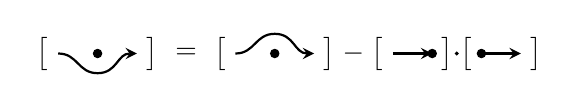
\begin{tikzpicture}[scale=0.5,>=stealth]
  \filldraw (-1,1) circle (3pt)
        (3.5,1) circle (3pt)
        (7.5,1) circle (3pt)
        (8.75,1)circle(3pt);
  \filldraw   (8.125,1) circle(1pt);
  \draw[thick,->] 
        (-2,1) ..controls (-1.5,1) and (-1.5,.5) ..(-1,.5)
             ..controls (-.5,.5) and (-.5,1) ..(0,1);
  \draw[thick,->] 
        (2.5,1) ..controls (3,1) and (3,1.5) ..(3.5,1.5)
             ..controls (4,1.5) and (4,1) ..(4.5,1);
  \draw[thick,->] (6.5,1) -- (7.5,1);
  \draw[thick,->] (8.75,1) -- (9.75,1);
  %symbols
  \draw (1.25,1) node {$=$}
      (5.5,1) node {$-$};
  \foreach \x in {-2,2.5,6.5,8.75}
  \draw (\x,1) node[left] {$\big[$};
  \foreach \x in {0,4.5,7.5,9.75}
  \draw   (\x,1) node[right] {$\big]$};     
\end{tikzpicture}
\caption{Relation in the algebra of paths}
\label{FigRelnPathAlg}
\end{figure}
  
  Let $\text{perm}:B_n\to S_n$ denote the homomorphism from $B_n$ to the symmetric group sending $\s_k$ to the simple transposition interchanging $k, k+1$. We will make use of the following.

  \begin{lem} For some $B\in B_n$ and $1\le i\ne j\le n$, consider $(\Phi_B^L)_{ij}\in \A_n$ as a polynomial expression in the (non-commuting) variables $\{a_{kl}, 1\le k\ne l\le n\}$. Writing $i'=\text{perm}(B)(i)$, every monomial in $(\Phi_B^L)_{ij}$ is a constant times $a_{i'i_1}a_{i_1i_2}\ldots a_{i_{l-1},j}$ for some $l\ge 0$, the monomial being a constant if $l=0$ and only if $i'=j$.
  \label{lem:monomial}
  \end{lem}
  \begin{proof}Include $B$ in $B_{n+1}$ and consider the isotopy class of the path $B\cdot c_{i,n+1}$ which begins at $i'$ and ends at $n+1$ (as $B$ does not interact with the $(n+1)$ strand. Applying the relation in Figure \ref{FigRelnPathAlg} to the path equates it with a sum (or difference) of another path with the same endpoints and a product of two paths, the first beginning at $i'$ and the other ending at $n+1$. A finite number of applications of this relation allows one to express the path as a polynomial in the $c_{kl}, 1\le k\ne l\le n$ where each monomial has the form $c_{i'i_1}\ldots c_{i_{l-1},j}$. The result then follows from the fact that $\phi_B(a_{i,n+1}) = \phi_B(F(c_{i,n+1})) = F(B\cdot c_{i,n+1})$.

  Alternatively, the statement follows from noting that (\ref{DefnPhiMap}) defining $\phi_{\s_k}$ has the desired property and that $\phi:B_n\to\text{Aut}(\A_n)$ is a homomorphism.
  \end{proof}

\subsection{Augmentations and augmentation rank}
\label{SecBG_AugRk}

  Let $S$ be a ring with 1, and consider it a differential graded algebra supported in grading 0, with trivial differential. Augmentations of $(\A,\partial)$ are DGA maps $(\A,\partial)\to (S,0)$. For our setting, if $B\in B_n$ is a braid representative of $K$, such a map corresponds precisely to a homomorphism $\epsilon:\A_n\otimes R_0\to\C$ such that $\epsilon$ sends each generator of $\mathcal I$ to zero (see Definition \ref{defn:HC_0}).

  \begin{defn}
  Suppose that $K$ is the closure of $B\in B_n$. An \emph{augmentation} of $K$ is a homomorphism $\epsilon: \A_n\otimes R_0\rightarrow \C$ such that each element of $\mathcal I$ is sent by $\epsilon$ to zero.
  \label{defn:Aug}
  \end{defn}

  A correspondence between augmentations and particular representations of the knot group $\pi_K$ were studied in \cite{Cor13a}. Recall that $\pi_K$ is generated by meridians. We may fix a meridian $m$ and generate $\pi_K$ by conjugates of $m$.

  \begin{defn}
  For any integer $r\ge1$, a homomorphism $\rho:\pi_K\to\text{GL}_r\C$ is a \emph{KCH representation} if there is a meridian $m$ of $K$ such that $\rho(m)$ is diagonalizable and has an eigenvalue of 1 with multiplicity $r-1$. We call $\rho$ a \emph{KCH irrep} if it is irreducible.
  \label{defn:KCHReps}
  \end{defn}

  In \cite{Ng08}, Ng describes an isomorphism between $HC_0(K)$ and an algebra constructed from elements of $\pi_K$. As discussed in \cite{Ng12} a KCH representation $\rho:\pi_K\to\text{GL}_r\C$ induces an augmentation $\epsilon_\rho$ of $K$. Given an augementation, the first author showed how to construct a KCH representation that induces it. In fact, we have the following rephrasing of results from \cite{Cor13a}.

  \begin{thm}[\cite{Cor13a}]
  Let $\epsilon:\A_n\otimes R_0\to\C$ be an augmentation with $\epsilon(\mu)\ne 1$. There is a KCH irrep $\rho:\pi_K\to\text{GL}_r\C$ such that $\epsilon_\rho=\epsilon$. Furthermore, for any KCH irrep $\rho:\pi_K\to\text{GL}_r\C$ such that $\epsilon_\rho = \epsilon$, $r$ equals the rank of $\epsilon({\bf A})$.
  \label{thm:AugKCH_Corresp}
  \end{thm}

  Considering Theorem \ref{thm:AugKCH_Corresp} we make the following definition.

  \begin{defn}
  The \emph{rank} of an augmentation $\epsilon:\A_n\otimes R_0\to\C$ with $\epsilon(\mu)\ne 1$ is the rank of $\epsilon({\bf A})$. Given a knot $K$, the \emph{augmentation rank of} $K$, denoted $\text{ar}(K)$, is the maximum rank among augmentations of $K$.
  \label{defn:AugRk}
  \end{defn}

  \begin{rem} The augmentation rank can be defined for target rings other than $\C$, but this paper only considers augmentations as in Definition \ref{defn:Aug}.
  \end{rem}

  It is the case that $\text{ar}(K)$ is well-defined. That is, given $K$ there is a bound on the maximal rank of an augmentation of $K$.

  \begin{thm}[\cite{Cor13b}] Given a knot $K\subset S^3$, if $g_1,\ldots,g_d$ are meridians that generate $\pi_K$ and $\rho:\pi_K\to\text{GL}_r\C$ is a KCH irrep then $r\le d$.
  \label{thm:DimBound}
  \end{thm}

  As in the introduction, if we denote the meridional rank of $\pi_K$ by $\text{mr}(K)$, then Theorem \ref{thm:DimBound} implies that $\text{ar}(K)\le\text{mr}(K)$. In addition, the geometric quantity $b(K)$ called the bridge index of $K$ is never less than $\text{mr}(K)$. Thus we have the following corollary:\todo[color=\ltgreen]{I made the inequality a corollary here}
    
\begin{cor}[\cite{Cor13b}] Given a knot $K\subset S^3$,
$$\text{ar}(K)\le\text{mr}(K)\le b(K)$$
\label{cor:DimBound}
\end{cor}

  As a result, to verify for $K$ that $\text{mr}(K)=b(K)$ it suffices to find an augmentation of $K$ with rank equal to $b(K)$. As we discuss in the next section, we will concern ourselves in this paper with a setting where $\text{ar}(K)=n$ and there is a braid $B\in B_n$ which closes to $K$. This is a special situation, since $b(K)$ is strictly less than the braid index for many knots.

\subsection{Finding augmentations}
\label{SecBG_AugExist}
  The following theorem concerns the behavior of the matrices $\Phi_B^L$ and $\Phi_B^R$ under the product in $B_n$. It is an essential tool for studying $HC_0(K)$ and will be central to our arguments.

  \begin{thm}[\cite{Ng05}, Chain Rule] Let $B,B'$ be braids in $B_n$. Then $\Phi_{BB'}^L = \phi_B(\Phi_{B'}^L)\cdot\Phi_B^L$ and $\Phi_{BB'}^R = \Phi_B^R\cdot\phi_B(\Phi_{B'}^R)$.
  \label{thm:ChainRule}
  \end{thm}

  The main result of this paper concerns augmentations with rank equal to the braid index of the knot $K$. Define the diagonal matrix $\Delta(B)=\text{diag}[(-1)^{w(B)},1,\ldots,1]$. The following statement follows from results in \cite[Section 5]{Cor13b}.\todo{but the theorem is marked Cor13a?}

  \begin{thm}[\cite{Cor13a}] If $K$ is the closure of $B\in B_n$ and has a rank $n$ augmentation $\epsilon:\A_n\otimes R_0\to\C$, then 
    \begin{equation}
    \epsilon(\Phi_B^L)=\Delta(B)=\epsilon(\Phi_B^R).
    \label{eqn:FindingAugs}
    \end{equation}
    Furthermore, any homomorphism $\epsilon:\A_n\to\C$ which satisfies (\ref{eqn:FindingAugs}) can be extended to $\A_n\otimes R_0$ to produce a rank $n$ augmentation of $K$. 
  \label{thm:RanknAugs}
  \end{thm}

  The proof of Theorem \ref{main} relies on this characterization of rank $n$ augmentations. That is, given a braid $B\in B_k$ with a rank $k$ augmentation $\epsilon:\cl A_k\to\C$, and $B'\in B_p$ with a rank $p$ augmentation $\epsilon':\cl A_p\to\C$ we show that $K(B,B')$ has a rank $kp$ augmentation by defining a homomorphism $\psi:\cl A_{kp}\to\cl A_k\otimes\cl A_p$ so that $(\epsilon\otimes\epsilon')\circ\psi$ satisfies (\ref{eqn:FindingAugs}) for the braid $B^{(p)}B'$.

  There is a symmetry on the matrices $\Phi_B^L$ and $\Phi_B^R$ that is relevant to the study of augmentations in this setting. Define an involution $x\mapsto\overline x$ on $\A_n$ (termed \emph{conjugation}) as follows: first set $\overline{a_{ij}}=a_{ji}$; then, for any $x,y\in\A_n$, define $\overline{xy}=\overline y\hspace*{1pt}\overline x$ and extend the operation linearly to $\A_n$. We have the following symmetry.

  \begin{thm}[\cite{Ng05}, Prop.\hspace*{-0.7pt} 6.2]For a matrix of elements in $\A_n$, let $\overline{M}$ be the matrix such that $\left(\overline M\right)_{ij} = \overline{M_{ij}}$. Then for $B\in B_n$, $\Phi_B^R$ is the transpose of $\overline{\Phi_B^L}$.
  \label{thm:Transpose}
  \end{thm}

  %Define $\A_n^{ab}$ to be the quotient of $\A_n$ by the ideal generated by $\{xy-yx | x,y\in\A_n\}\cup\{a_{ij}-a_{ji} | i\ne j\}$. Any homomorphism $\epsilon:\A_n\to\C$ such that $\epsilon(a_{ij}-a_{ji})=0$ for all $i\ne j$ determines a homomorphism $\epsilon:\A_n^{ab}\to\C$. As a consequence, Theorems \ref{thm:RanknAugs} and \ref{thm:Transpose} imply that finding $\epsilon:\A_n\to\C$ such that $\epsilon(a_{ij}-a_{ji})=0$ and satisfying $\epsilon(\Phi_B^L) = \Delta(B)$ suffices to determine a rank $n$ augmentation. There do exist braids $B\in B_n$ and homomorphisms $\epsilon:\A_n\to\C$ satisfying (\ref{eqn:FindingAugs}), such that $\epsilon$ does not descend to $\A_n^{ab}$. However, to date every such braid $B\in B_n$ that has been found, also admits a homomorphism satisfying (\ref{eqn:FindingAugs}) that does descend to $\A_n^{ab}$. 

\todo[color=\ltgreen,inline]{It may be appropriate here to indicate that $\text{ar}(K)<\text{mr}(K)$ sometimes (maybe in previous subsection), and talk about the 2-cable of the trefoil that does not have $\text{ar}(K,\mathbb C)=4$}

%%%%%%%%%%%%%%%%%%%%%%%%%%%%%%%%%%%%%%%%%%%%%%%%%%%%%%%%%%%%%%%%%%%%%%%%%%%%%%%%%%%%%%%%%%%%%%%%%%%%%%%%%%%%%%%%%%%%%%%%%%%%%%%%%%%%%%%%%%%%
%%%%%%%%%%%%%%%%%%%%%%%%%%%%%%%%%%%%%%%%%%%%%%%%%%%%%%%%%%%%%%%%%%%%%%%%%%%%%%%%%%%%%%%%%%%%%%%%%%%%%%%%%%%%%%%%%%%%%%%%%%%%%%%%%%%%%%%%%%%%

\section{Main Results}
\label{SecMain}
\todo[color=\ltblue,inline]{figure out this two tensor products nonsense}

\todo[inline]{how do I bring in equations to fit margins?}

\subsection{Proof of Theorem \ref{main}}
\label{SecProofMain}
In this section we prove our main result, which we now recall. We will use the notation of the Theorem throughout Section \ref{SecMain}.

\newtheorem*{main}{Theorem \ref{main}}
\begin{main}
If $B$ is a $k$-braid such that $\ar(B)=k$ and $B'$ a $p$-braid such that $\ar(B')=p$ then $\ar(K(B,B'))=kp$.
\end{main}

%As we saw in the introduction, Theorem \ref{main} has an immediate corollary, which follows from Corollary \ref{cor:DimBound} and Theorem 1.3 from \cite{Cor13b}:

%\newtheorem*{cor:iteratedCables}{Corollary \ref{cor:iteratedCables}}
%\begin{cor:iteratedCables}
%Let $T$ be an iterated torus knot, and suppose it arises from taking $(p_i,q_i)$-cables such that $p_i<q_i$ for all $i$. Then $\mr(T) = b(T)$.
%\end{cor:iteratedCables}

As mentioned in the previous section, we prove Theorem \ref{main} by defining an algebra map $\psi\colon \A_{pk} \rightarrow \A_k\otimes \A_p$. The key point is that $\psi(\Phi_{K(B,B')}^L)$ decomposes {\color{red} (wc?)} in such a way that we may compose with an augmentation from each of $B$ and $B'$ to obtain a homomorphism satisfying (\ref{eqn:FindingAugs}). The decomposition is described by Proposition \ref{psiofbp} will follow from Lemmas \ref{commutes} and \ref{basecase}, the former following from a calculation (Lemma \ref{Sigma_n}) and the latter depending on the former. We begin with the definition of $\psi$ and statement of Proposition \ref{psiofbp}, followed by the proof of Proposition \ref{psiofbp} and Lemmas \ref{commutes},\ref{basecase}, and \ref{Sigma_n}.


%Among other things, this theorem implies that iterated cables of torus knots have meridional rank equal to their bridge number. \todo[color=\ltblue]{braid rep've info needed to make well-defined} Consider a $(r,s)$-torus knot $T$ with $\gcd(r,s) = 1$ and $r<s$. $T$ has bridge number $r$ and is the closure of a braid $B$ on $r$ strands, and since all torus knots have bridge number equal to their augmentation rank (\todo[color=\ltblue]{cite cornwell}), we have that there exists an augmentation $\epsilon_T\colon \A_r\rightarrow \C$\todo[color=\ltblue]{finish this}. . given by the braid sum of $T^{(p)}$ with a braid who's first $p$ strands form a torus knot with bridge number (and therefore augmentation rank) equal to $p$ and such that $w(T)$ is even (i.e. a $(p,q)$ torus knot, where $\gcd(p,q) = 1$, $p<q$, and $pq-q$ is even). Theorem \ref{main} then says that this cable has augmentation rank equal to its braid index, implying that its meridional rank is equal to its bridge number. Furthermore, we can iterate this process, taking cables of the resulting knots with augmentation rank, bridge number, and braid index all equal.\todo[color=\ltblue]{prob from Kirby list should be mentioned here}

For each $1\le i\le pk$ let $q_i\ge0$ and $0 < r_i \le p$ be the integers such that $i = q_ip + r_i$. For each generator $a_{ij}, 1\le i\ne j\le kp$, define

\begin{equation}
\psi(a_{ij}) =
  \begin{cases}
         1\otimes a_{r_ir_j} & \colon q_i = q_j\\
         a_{q_i+1,q_j+1}\otimes 1 & \colon r_i = r_j\\
         0 & \colon (q_i-q_j)(r_i-r_j)<0\\
         a_{q_i+1,q_j+1}\otimes a_{r_ir_j} & \colon (q_i-q_j)(r_i-r_j)>0\\
  \end{cases},
  \label{defn:psi}
\end{equation}

\noindent which determines an algebra map $\psi\colon \A_{pk} \rightarrow \A_k\otimes \A_p$. Note that if $\psi(a_{ij}) \in 1\otimes \A_p$ then $q_i = q_j$ or $a_{ij}\in\ker\psi$. Also, if we extend conjugation to $\A_k\otimes\A_p$ by applying it to each factor, then $\psi(\overline{a_{ij}}) = \overline{\psi(a_{ij})}$. We have the following proposition.


\begin{prop}\label{psiofbp}
For any braid $B$, $\psi\left(\Phi_{B^{(p)}}^L\right) = \left(\left(\Phi_B^L\right)_{ij}\otimes 1\right)\otimes I_p$ and $\psi\left(\Phi_{B^{(p)}}^R\right) = \left(\left(\Phi_B^R\right)_{ij}\otimes 1\right)\otimes I_p$\todo[color=\ltblue]{make consistent throughout paper}
\end{prop}


Note that here we mean the tensor product of $\Phi_B^L$ and $I_p$ as matrices, not as linear maps, while the tensor product of $\left(\Phi_B^L\otimes I_p\right)_{ij}$ and $1$ is a tensor product of algebra elements, so that if we divide the matrix $\psi(\Phi_{B^{(p)}}^L)$ into $k^2$ $p\times p$ blocks, the $ij$th block is $\left((\Phi_B^L)_{ij}\otimes 1\right)I_p$.

It turns out that instead of $\psi$ we could have defined a simpler homomorphism $\rho\colon \A_{pk}\rightarrow \A_k$ that would take $a_{ij}$ to $a_{q_{i+1},q_{j+1}}$ if $r_i=r_j$ and 0 otherwise, and Proposition \ref{psiofbp} would still be true (this follows from the same ideas used in the proof of Proposition \ref{psiofbp}). The advantage of $\psi$ is that it doesn't send $a_{ij}$ to 0 if $q_i=q_j$, a fact which will be important in the proof of Theorem \ref{main}.


\begin{proof}[Proof of Theorem \ref{main}]
By Theorem \ref{thm:RanknAugs} there exist augmentations $\epsilon_k\colon \A_k\otimes R_0 \rightarrow \C$ and $\epsilon_p\colon \A_p\otimes R_0 \rightarrow \C$, for the closures of $B,B'$ respectively, such that $\epsilon_k\left(\Phi_B^L\right) = \epsilon_k\left(\Phi_B^R\right) = \Delta(B)$ and $\epsilon_p\left(\Phi_{B'}^L\right) = \epsilon_p\left(\Phi_{B'}^R\right) = \Delta(B')$. Theorem \ref{thm:RanknAugs} also implies that it suffices to prove that there exists an augmentation $\epsilon\colon \A_{pk}\otimes R_0\rightarrow \C$ such that $\epsilon\left(\Phi_{B^{(p)}B'}^L\right) = \epsilon\left(\Phi_{B^{(p)}B'}^R\right) = \Delta(B^{(p)}B')$.

Below we will define a homomorphism $\delta\colon\A_p\rightarrow \C$ such that $\delta = \pm \epsilon_p$, the sign depending on the parity of $w(B)$ and $p$. Let $\pi\colon \C\otimes \C \rightarrow \C$ be the multiplication isomorphism $a\otimes b\mapsto ab$. Our desired map is defined by $\epsilon = \pi\circ(\epsilon_k\otimes\delta)\circ\psi$.

The Chain Rule theorem gives that
\begin{equation}
\pi\circ(\epsilon_k\otimes\delta)\circ\psi\left(\Phi_{B^{(p)}B'}^L\right) = \pi\circ(\epsilon_k\otimes\delta)\psi\left(\phi_{B^{(p)}}\left(\Phi_{B'}^L\right)\right)\psi\left(\Phi_{B^{(p)}}^L\right)
\label{eqn1MainPf}
\end{equation}

Consider the homomorphism $\phi_{B^{(p)}}$ through the description given in Section \ref{SecBG_KCHdef}. As each $a_{ij}, 1\le i\ne j\le p$, is represented by the isotopy class $c_{ij}$, and the leftmost $p$ punctures are moved as one block by the action of $B^{(p)}$ on $D$, there is an $0\le m<k$ so that $\phi_{B^{(p)}}(a_{ij})=a_{i+mp,j+mp}$ for each $i,j$ in this range. As $\psi(a_{i + mp, j+mp})=1\otimes a_{ij}$,

$$\psi\left(\phi_{B^{(p)}}\left(\Phi_{B'}^L\right)\right) = \left(1\otimes \left(\Phi_{B'}^L\right)_{ij}\right)$$

\noindent By Proposition \ref{psiofbp}, we have that 

$$\psi\left(\Phi_{B^{(p)}}^L\right) = \left(\left(\Phi_B^L\right)_{ij}\otimes 1\right)\otimes I_p = \left(\left(\Phi_B^L\otimes I_p\right)_{ij}\otimes 1\right)$$

\noindent Returning to the right hand side of (\ref{eqn1MainPf}) we get
\begin{align*}
\pi\circ(\epsilon_k\otimes\delta)\left(\psi\left(\phi_{B^{(p)}}\left(\Phi_{B'}^L\right)\right)\psi\left(\Phi_{B^{(p)}}^L\right)\right)
    & = \pi\circ(\epsilon_k\otimes\delta)\left(\left(1\otimes \left(\Phi_{B'}^L\right)_{ij}\right)\left(\left(\Phi_B^L\otimes I_p\right)_{ij}\otimes 1\right)\right)\\
    & = \delta\left(\Phi_{B'}^L\right)\left(\Delta(B)\otimes I_p\right)
\end{align*}


We are done if we can define $\delta$ so that $\delta\left(\Phi_{B'}^L\right)\left(\Delta(B)\otimes I_p\right) = \Delta(B^{(p)}B')$. When $w(B)$ is even we simply let $\delta = \epsilon_p$. Since $w(B)$ is even, $w(B^{(p)})$ is also. Hence $\Delta(B)=I_k$ and $\epsilon_p\left(\Phi_{B'}^L\right) = \Delta(B') = \Delta(B^{(p)}B')$ and the result follows.

Suppose that $w(B)$ is odd. We define $g\colon \{1,\ldots,p\}\rightarrow \{\pm 1\}$ as follows. Let $x_1 = 1$, and $x_l = \perm(B')(x_{l-1})$ for $1<l\le p$. Since the first $p$ strands of $B'$ close to a knot, $\perm(B')$ is given by the $p$-cycle $(x_1x_2\ldots x_p)$. If $p$ is even, we let $g(x_1) = 1$, and $g(x_l) = -g(x_{l-1})$ for $1<l\le p$. If $p$ is odd, let $g(x_1) = g(x_2) = 1$ and $g(x_l) = -g(x_{l-1})$ for $2<l\le p$.

 Define $\delta: \A_p\to \C$ by setting $\delta(a_{ij}) = g(i)g(j)\epsilon_k(a_{ij})$ for $1\le i\ne j\le p$. Fix $i,j$ and consider a monomial $M$ in $\left(\Phi_{B'}^L\right)_{ij}$, which is constant if $i>p$ or $j>p$ so that $\delta(M)$ is defined. If $i,j\le p$, then writing $i'=\text{perm}(B')(i)$, Proposition \ref{lem:monomial} implies $M=c_{ij}a_{i',j_1}a_{j_1,j_2}\ldots a_{j_m,j}$ for some $j_1,\ldots j_m\in \{1,\ldots,p\}$, possibly being constant only if $i'=j$, implying that 

$$\delta(M) = g(i')g(j)\left(\prod_{k=1}^m g(j_k)^2\right)\epsilon_p(M) = g(i')g(j)\epsilon_p(M).$$

\noindent Note, when $M$ is constant then $\delta(M) = M = g(i')g(j)\epsilon_p(M)$ since $i'=j$. Since this holds for each monomial, we have that

$$\delta\left(\left(\Phi_{B'}^L\right)_{ij}\right) = g(i')g(j)\epsilon_p\left(\left(\Phi_{B'}^L\right)_{ij}\right).$$

When $p$ is even, $w(B^{(p)})$ is also even and so the opposite parity of $w(B)$. Our definition of $g$ gives $\delta\left(\left(\Phi_{B'}^L\right)_{ii}\right) = -\epsilon\left(\left(\Phi_{B'}^L\right)_{ii}\right)$ for $i\le p$. Thus 

$$\delta\left(\Phi_{B'}^L\right) = 
\left( \begin{array}{ccc}
(-1)^{w(B')+1} & 0 & 0 \\
0 & -I_{p-1} & 0 \\
0 & 0 & I_{(k-1)p} \end{array} \right)
$$
\noindent and therefore
$$
\delta\left(\Phi_{B'}^L\right)\left(\Delta(B)\otimes I_p\right) = \diag[(-1)^{w(B) + w(B') + 1},1\ldots 1] = \Delta(B^{(p)}B')
$$
\noindent as desired.

Since $p$ is odd, $w(B^{(p)})$ is odd and therefore the same parity of $w(B)$. Our definition of $g$ gives that $\delta\left(\left(\Phi_{B'}^L\right)_{11}\right) = \epsilon\left(\left(\Phi_{B'}^L\right)_{11}\right)$ and $\delta\left(\left(\Phi_{B'}^L\right)_{ii}\right) = -\epsilon\left(\left(\Phi_{B'}^L\right)_{ii}\right)$ for $1<i\le p$, so 

$$\delta\left(\Phi_{B'}^L\right) = 
\left( \begin{array}{ccc}
(-1)^{w(B')} & 0 & 0 \\
0 & -I_{p-1} & 0 \\
0 & 0 & I_{(k-1)p} \end{array} \right)
$$
\noindent and therefore
$$
\delta\left(\Phi_{B'}^L\right)\left(\Delta(B)\otimes I_p\right)= \diag[(-1)^{w(B) + w(B')},1\ldots 1] = \Delta(B^{(p)}B')
$$
\noindent as desired. 

There is little difference in the proof that $\epsilon(\Phi_{B^{(p)}}^R) = \Delta(B^{(p)}B')$, except that monomials in $(\Phi_{B'}^R)_{ij}$ are of the form $c_{ij}a_{i,j_1}a_{j_1,j_2}\cdots a_{j_k,j'}$ where $j'=\text{perm}(B')(j)$. Applying Theorem \ref{thm:RanknAugs} now completes the proof.
%Similarly, we have that
%$$
%\pi\circ(\epsilon_k\otimes\delta)\circ\psi\left(\Phi_{B^{(p)}B'}^R\right) = \pi\circ(\epsilon_k\otimes\delta)\left(\left(\left(\Phi_B^R\otimes I_p\right)_{ij}\otimes 1\right)\left(1\otimes \left(\Phi_{B'}^R\right)_{ij}\right)\right)
%$$
%but since $\epsilon_k\left(\Phi_B^L\right) = \epsilon_k\left(\Phi_B^R\right)$ and $\epsilon_p\left(\Phi_{B'}^L\right) = \epsilon_p\left(\Phi_{B'}^R\right)$, in each case above we have
%\begin{align*}
%\pi\circ(\epsilon_k\otimes\delta)\left(\left(\left(\Phi_B^R\otimes I_p\right)_{ij}\otimes 1\right)\left(1\otimes \left(\Phi_{B'}^R\right)_{ij}\right)\right) &= \pi\circ(\epsilon_k\otimes\delta)\left(\left(\left(\Phi_B^L\otimes I_p\right)_{ij}\otimes 1\right)\left(1\otimes \left(\Phi_{B'}^L\right)_{ij}\right)\right)\\
%&= \Delta\left(B^{(p)}B'\right)
%\end{align*}
\end{proof}

\subsection{Supporting Lemmas}
\label{SecLemmasMain}

\noindent We will use the following two lemmas in our proof of Proposition \ref{psiofbp}. Figure \ref{FigCommutes} demonstrates an example for Lemma \ref{commutes}, showing that $\psi(\phi_{\Sigma^{(2)}_2}(a_{24})) = (\phi_{\s_2}\otimes\id)(\psi(a_{24}))$. Note that in the figure we condense elements such as $a_{13}\otimes 1$ to $a_{13}$ in order to make the notation cleaner.


\begin{lem}\label{commutes}
$\psi(\phi^{\pm}_{\Sp_n}(a_{ij})) = (\phi_{\s_n^{\pm 1}} \otimes \id)(\psi(a_{ij}))$ for all $1\le n < k$, $1 \le i,j \le pk$.
\end{lem}

\begin{lem}\label{basecase}
$\psi\left(\Phi_{{\Sp_n}^{\pm}}^L\right) = \left(\left(\Phi_{\s_n^{\pm 1}}^L\right)_{ij}\otimes 1\right)\otimes I_p$
\end{lem}


%FigCommutes
\begin{figure}[ht]
\begin{tikzpicture}[scale=0.245,>=stealth]
\foreach \y in {0}
	\foreach \p in {0,1,3,4,6,7} \filldraw (\p,\y) circle (1.5pt);
	
\foreach \a in {3.5}
	\foreach \b in {-3.5,-2.5,-.5,.5,2.5,3.5} \filldraw (\a+\b,-3) circle (1.5 pt);
	
\foreach \a in {3.5,15.5,27.5,39.5}
	\foreach \b in {-3.5,-2.5,-.5,.5,2.5,3.5} \filldraw (\a+\b,-6) circle (1.5 pt);

\draw (-3.2,0) node {{\Large $\psi(\phi_{\Sigma^{(2)}_2}($}};
\draw (8,0) node {{\Large $))$}};

\oarc{1}{0}{4}{0};
%\draw[->,thick] (1,1) ..controls (1.2,1.7) and (6.8,1.7) .. (7,1);
%\x = 12
%\draw[->,thick] (\c + 1,1) ..controls (\c + 1.2,.3) and (\c + 4.8,.3) .. (\c + 5,1);


\draw[->,thick] (1,-3) ..controls (1.5,-3.75) and (4.5,-3.75) .. (5,-3)
								  ..controls (5.5,-2.25) and (6.5,-2.25) .. (7,-3);


\draw (-3.2,-3) node {{$=$}};
\draw (-1.2,-3) node {{\Large $\psi($}};
\draw (7.7,-3) node {{\Large $)$}};

\draw (-3.2,-6) node {{$=$}};
\draw (-1.2,-6) node {{\Large $\psi($}};
\draw (44,-6) node {{\Large $)$}};

\oarc{1}{-6}{3}{-6};
\oarc{3}{-6}{4}{-6};
\oarc{4}{-6}{7}{-6};

\oarc{13}{-6}{16}{-6};
\oarc{16}{-6}{19}{-6};

\draw (9.5,-6) node {{$-$}};
\draw (21.5,-6) node {{$-$}};

\oarc{25}{-6}{27}{-6};
\oarc{27}{-6}{31}{-6};

\oarc{37}{-6}{43}{-6};

%\draw (33.5,-6) node {{$+$}};

\draw (-3.2,-9) node {{$=$}};

\foreach \x in {3.5,13.5}
	\foreach \c in {-1,0,1} \filldraw (\x + \c,-9) circle(1.5pt);
	

\draw (-1.5,-9) node {{0}};
\draw (1,-9) node {{$-$}};

\oarc{2.5}{-9}{3.5}{-9};
\oarc{3.5}{-9}{4.5}{-9};

\draw (6,-9) node {{$-$}};

\draw (8.5,-9) node {{0}};

\oarc{12.5}{-9}{14.5}{-9};

\draw (11,-9) node {{$+$}};

\draw (-3.2,-12) node {{$=$}};
\draw (-.5,-12) node {{\Large $\phi_{\s_2}($}};
\draw (3.9,-12) node {{\Large $)$}};

\foreach \x in {1.2,2.2,3.2} \filldraw (\x,-12) circle(1.5pt);

\oarc{1.2}{-12}{2.2}{-12};

\end{tikzpicture}
\caption{Computing $\psi(\phi_{\Sp_2}(a_{24}))$}
\label{FigCommutes}
\end{figure}




%Proof of psiofbp
\begin{proof} [Proof of Proposition \ref{psiofbp}]
Let $B = \s_{n_1}^{q_1}\cdots\s_{n_r}^{q_r}$, where $1\le n_i<k$ and $q_i = \pm 1$. We will prove the proposition by induction on $r$. The base case is already taken care of by Lemma \ref{basecase}. Suppose that the proposition holds for braids of length $r-1$. Let $B' =\s_{n_1}^{q_1}\cdots\s_{n_{r-1}}^{q_{r-1}}$ Then by the Chain Rule and Lemmas \ref{commutes} and \ref{basecase}, we have that
\begin{align*}
\psi\left(\Phi_{B^{(p)}}^L\right) &= \psi\left(\phi_{B'^{(p)}}\left(\Phi_{\Sigma^{q_r(p)}_{n_r}}^L\right)\cdot\Phi_{B'^{(p)}}^L\right)\\
&= \left(\phi_{B'}\otimes\id\right)\left(\psi\left(\Phi_{\Sigma^{q_r(p)}_{n_r}}^L\right)\right)\cdot \left(\left(\Phi_{B'}^L\right)_{ij}\otimes 1\right)\otimes I_p\\
&= \left(\phi_{B'}\otimes\id\right)\left(\left(\left(\Phi_{\s_{n_r}^{q_r}}^L\right)_{ij}\otimes 1\right)\otimes I_p\right)\cdot \left(\left(\Phi_{B'}^L\right)_{ij}\otimes 1\right)\otimes I_p\\
&= \left(\left(\Phi_{B}^L\right)_{ij}\otimes 1\right)\otimes I_p.
\end{align*}
In addition, $\psi\left(\Phi_{B^{(p)}}^R\right) = \left(\left(\Phi_{B}^R\right)_{ij}\otimes 1\right)\otimes I_p$, since $\Phi_B^R = \overline{\Phi_B^L}^t$ and $\psi(\overline{a_{ij}}) = \overline{\psi(a_{ij})}$.
\end{proof}


In the proof of Lemmas \ref{commutes} and \ref{basecase}, we will make use of some calculations of $\phi_B(a_{ij})$ for simple braids $B$. Recall that $\tau_{m,l} = \s_m\s_{m+1}\cdots\s_{m+l-1}$. It can easily be checked that for all $1\le m < n$, $1\le l \le n - m$, $i<j$
\begin{equation}\label{tau}
\phi_{\tau_{m,l}}(a_{ij}) =
\left\{
     \begin{array}{lr}
       a_{i+1,j+1} & \colon m\le i<j< m+l\\
       a_{i-l,j} & \colon m<m+l=i<j\\
       a_{i,j-l} & \colon i<m<m+l=j\\
       a_{i+1,j-l} & \colon m\le i < j = m+l\\
       a_{i,j+1}-a_{i,m}a_{m,j+1} & \colon i<m\le j< m+l\\
       a_{i+1,j}-a_{i+1,m}a_{m,j} & \colon m\le i< m+l<j\\
       a_{ij} & \colon \textnormal{otherwise}
     \end{array}
\right.
\end{equation}

\noindent We also make the following definition

\noindent Let $X\subseteq \{1,\ldots,n\}$, and write the elements of a subset $Y\subseteq X$ as $y_1<\ldots <y_k$. Define
$$
 A(i,j,X) = \sum_{Y\subseteq X}(-1)^{|Y|}a_{iy_1}a_{y_1y_2}\cdots a_{y_kj}
$$
and
$$
 A'(i,j,X) = \sum_{Y\subseteq X}(-1)^{|Y|}a_{iy_k}a_{y_ky_{k-1}}\cdots a_{y_1j}
$$



\noindent and have the following lemma

%Lemma Sigma_n
\begin{lem}\label{Sigma_n}
Suppose $i<j$. Let $\kappa_{m,l} = \t_{m+l-1,p}\t_{m+l-2,p}\cdots\t_{m,p}$, and let $X_{m,l} = \{m,\ldots,m+l-1\}$. Then
\todo[color=\ltblue]{check}
$$
\phi_{\kappa_{m,l}}(a_{ij}) =
\left\{
     \begin{array}{lr}
       a_{i-p,j-p} & \colon m+p\le i<j< m+l+p\\
       a_{i-p,j} &\colon m+p\le i< m+l+p\le j\\
       a_{i,j-p} & \colon i<m<m+p\le j<m+l+p\\
       a_{i+l,j+l} &\colon m\le i<j<m+p\\
       A'(i+l,j-p,X_{m,l}\setminus (j-p)) & \colon m\le i<m+p\le j <m+l+p\\
       A(i,j+l,X_{m,l}) & \colon i<m\le j <m+p<m+l+p\\
       A'(i+l,j,X_{m,l}) & \colon m\le i <m+p<m+l+p\le j\\
       a_{ij} & \colon \textnormal{otherwise}
     \end{array}
\right.
$$
\end{lem}

\noindent Note that letting $l=p$ and $m=(n-1)p+1$ gives us $\phi_{\Sigma_n^{(p)}}(a_{ij})$ when $i<j$ as a special case. Letting $X_n^{(p)} = \{(n-1)p+1,\ldots,np\}$, we have

$$
\phi_{\Sigma_n^{(p)}}(a_{ij}) =
\left\{
     \begin{array}{lr}
       a_{i-p,j-p} & \colon np< i<j\le (n+1)p\\
       a_{i-p,j} &\colon np< i\le (n+1)p< j\\
       a_{i,j-p} & \colon i\le(n-1)p<np< j\le(n+1)p\\
       a_{i+p,j+p} &\colon (n-1)p< i<j\le np\\
       A'(i+p,j-p,X_n^{(p)}\setminus (j-p)) & \colon (n-1)p< i\le np< j \le (n+1)p\\
       A(i,j+p,X_n^{(p)}) & \colon i\le(n-1)p< j \le np<(n+1)p\\
       A'(i+p,j,X_n^{(p)}) & \colon (n-1)p< i \le np<(n+1)p< j\\
       a_{ij} & \colon \textnormal{otherwise}
     \end{array}
\right.
$$


%proof of commutes
\begin{proof} [Proof of Lemma \ref{commutes}]
We need only show that $\psi(\phi_{\Sp_n}(a_{ij})) = (\phi_{\s_n} \otimes \id)(\psi(a_{ij}))$. The equality $\psi\left(\phi_{{\Sp_n}^{\textrm{-}1}}\left(a_{ij}\right)\right) = \left(\phi_{\s_n^{-1}}\otimes\id\right)(\psi(a_{ij}))$ immediately follows.

Furthermore, $\phi_B(\overline{a_{ij}}) = \overline{\phi_B(a_{ij})}$ and $\psi(\overline{a_{ij}}) = \overline{\psi(a_{ij})}$, so it suffices to prove the lemma for $\Sp_n$ in the case where $i<j$.

With these restrictions, we then break the statement up into the cases from Lemma \ref{Sigma_n}, from which the first four cases as well as the last case can be checked easily. Consider the sixth case. Lemma \ref{Sigma_n} gives that
$$\psi\left(\phi_{\Sp_n}(a_{ij})\right) = \sum_{Y\subseteq \{np-p+1,\ldots,np\}}(-1)^{|Y|}\psi\left(a_{iy_1}a_{y_1y_2}\cdots a_{y_k,j+p}\right)$$
%&= \psi\left(A(i,j+p,\{np-p+1,\ldots,np\})\right)\\


Let $\a_i  = np-p+r_i$. Note that if $y_1<\a_i$ then $\psi(a_{iy_1}) = 0$, and if $y_k>\a_j$ then $\psi(a_{y_kj}) = 0$, so the sum on the right hand side can be taken over $Y\subseteq\{\a_i,\a_i+1,\ldots,\a_j\}$. Then we manipulate the sum to get\todo{do I need to explain what I'm doing here?}

\begin{align*}
& \sum_{Y\subseteq \{\a_i,\ldots,\a_j\}}(-1)^{|Y|}\psi\left(a_{iy_1}a_{y_1y_2}\cdots a_{y_k,j+p}\right)\\
&= \psi\left(a_{i,j+p} - a_{i,\a_i}a_{\a_i,j+p}\right)\\
& \;\;\;\;+ \sum_{y=\a_i+1}^{\a_j}\sum_{Y\subseteq \{y+1,\ldots,\a_j\}}(-1)^{|Y|+1}\psi\left(a_{iy}a_{yy_1}\cdots a_{y_k,j+p}\right) + (-1)^{|Y|}\psi\left(a_{i,\a_i}a_{\a_i,y}a_{yy_1}\cdots a_{y_k,j+p}\right)\\
&= \psi\left(a_{i,j+p} - a_{i\a_i}a_{\a_i,j+p}\right)\\
& \;\;\;\;+ \sum_{y=\a_i+1}^{\a_j}\sum_{Y\subseteq \{y+1,\ldots,\a_j\}}(-1)^{|Y|}\psi\left(a_{i,\a_i}a_{\a_i,y} - a_{iy}\right)\psi\left(a_{yy_1}\cdots a_{y_k,j+p}\right)\\
\end{align*}



Note that $r_i = r_{\a_i}$ and since we're in the sixth case we have $(n-1)p<j\le np$, so $q_{\a_i}=q_y$. Thus $\psi(a_{i,\a_i}) = a_{q_i+1,q_{\a_i}+1}\otimes 1 = a_{q_i+1,q_y+1}\otimes 1$ and $\psi(a_{\a_i,y}) = 1\otimes a_{r_{\a_i},r_y} = 1\otimes a_{r_i,r_y}$, so we have
$$\psi(a_{i,\a_i}a_{\a_i,y} - a_{iy}) = \left(a_{q_i+1,q_y+1}\otimes 1\right)\left(1\otimes a_{r_i,r_y}\right) - a_{q_i+1,q_y+1}\otimes a_{r_i,r_y} = 0$$
Thus the right hand side reduces to 
$$\psi\left(a_{i,j+p} - a_{i\a_i}a_{\a_i,j+p}\right)$$

\begin{rem}
The fact that $\psi(a_{i,\a_i}a_{\a_i,y} - a_{iy}) = 0$ and $\psi$ behaves similarly for the analogous terms in the other cases is the key to this proof working, and $\psi$ is defined the way it is mainly so that this will be true. As we hinted at earlier, the homomorphism $\rho\colon \A_{pk}\rightarrow \A_k$ defined to send $a_{ij}$ to $a_{q_i+1,q_j+1}$ if $r_i=r_j$ and to 0 otherwise would also send these terms to 0, so Proposition \ref{psiofbp} would still be true with $\rho$ used in the place of $\psi$. We will need $\psi$ for the proof of the main result, however.
\end{rem}

\noindent Note that, since we're in the sixth case, $q_j + 1 = n$. If $r_i = r_j$, then 
$$\psi\left(a_{i,j+p} - a_{i\a_i}a_{\a_i,j+p}\right) = \left(a_{q_i+1,n+1} - a_{q_i+1,n}a_{n,n+1}\right)\otimes 1 = (\phi_{\s_n} \otimes \id)(\psi(a_{ij}))$$
If $r_i < r_j$, then
\begin{align*}
\psi\left(a_{i,j+p} - a_{i\a_i}a_{\a_i,j+p}\right) &= \left(a_{q_i+1,n+1}\otimes a_{r_ir_j} - a_{q_i+1,n}a_{n,n+1}\otimes a_{r_ir_j}\right)\\
&= \left(a_{q_i+1,n+1} - a_{q_i+1,n}a_{n,n+1}\right)\otimes a_{r_ir_j}\\
&= (\phi_{\s_n} \otimes \id)(\psi(a_{ij}))
\end{align*}
Finally, if $r_i > r_j$, then
$$\psi\left(a_{i,j+p} - a_{i\a_i}a_{\a_i,j+p}\right) = 0 = (\phi_{\s_n} \otimes \id)(\psi(a_{ij}))$$

The proof for the seventh case goes exactly as the proof for the sixth case except with all $i$'s replaced with $i+p$, all $(j+p)$'s replaced with $j$, all $y_i$'s replaced with $y_{k+1-i}$, and with $\a_i$ and $\a_j$ swapped. The proof for the fifth case goes exactly as the proof for the seventh, except that $j-p$ is removed from the set that $Y$ is a subset of in all the sums.\todo[color=\ltblue]{check this}
\end{proof}



%proof of basecase
\begin{proof} [Proof of Lemma \ref{basecase}]\todo[color=\ltblue]{check}
First we will prove the lemma for $\Sp_n$. Extend $\psi$ to be a map from the free $\A_{pk}$-module generated by elements $\{a_{i*}|1\le i\le pk\}$ to the free module over $\A_{k}\otimes \A_{p}$ generated by $\{a_{i*}|1\le i\le k\}$ \todo[color=\ltgreen]{do you want $k$ here, or $pk$?} by defining $\psi(aa_{i*}) = \psi(a)a_{i*}$ for any $a\in\A_{pk}$ and then extending by linearity. 

Now the statement of the lemma is equivalent to saying that for all $1\le i\le pk$, the coefficient of $a_{j*}$ in $\psi\left(\phi_{\Sp_n}(a_{i*})\right)$ is equal to 0 unless $r_j = r_i$, in which case it is equal to the coefficient of $a_{q_j+1,*}$ in $\phi_{\s_n}(a_{q_i+1,*})$. If $q_i + 1 \ne n$, this fact can be easily checked. In the case that $q_i + 1 = n$, we have that
$$\psi\left(\phi_{\Sp_n}(a_{i*})\right) = \psi\left(A(i+p,*,\{np-p+1,\ldots,np\}\right)$$
\noindent which is equal to
$$\psi(a_{i+p,*} - a_{i+p,\a_i}a_{\a_i,*}) = a_{i+p,*} - (a_{q_i+2,q_i+1}\otimes 1)a_{\a_i,*}$$
by the same argument that was used in Lemma \ref{commutes}. Since in this case $\alpha_i=(n-1)p+r_i = i$, the coefficients of $a_{i+p,*}$ and $a_{\a_i,*}=a_{i*}$ are equal to the coefficients of $a_{n+1,*}$ and $a_{n*}$ respectively in $\phi_{\s_n}(a_{q_i+1,*})$, so we have $\psi\left(\Phi_{\Sp_n}^L\right) = \left(\left(\Phi_{\s_n}^L\right)_{ij}\otimes 1\right)\otimes I_p$.

Using this fact, the Chain Rule, and Lemma \ref{commutes}, we have
\begin{align*}
\left(\left(I_{pk}\right)_{ij}\otimes 1\right) &= \psi\left(\Phi_{\SpM_n\Sp_n}^L\right)\\
&= \psi\left(\phi_{\SpM_n}\left(\Phi_{\Sp_n}^L\right)\right)\psi\left(\Phi_{\SpM_n}^L\right)\\
&= \left(\phi_{\s_n^{-1}}\otimes \id\right)\left(\left(\left(\Phi_{\s_n}\right)_{ij}\otimes 1\right)\otimes I_p\right)\psi\left(\Phi_{\SpM_n}^L\right)\\
\end{align*}
But note that the Chain Rule also gives that $\left(\left(\Phi_{\s_n^{-1}}^L\right)_{ij}\otimes 1\right)\otimes I_p$ is the inverse of $\left(\phi_{\s_n^{-1}}\otimes \id\right)\left(\left(\left(\Phi_{\s_n}\right)_{ij}\otimes 1\right)\otimes I_p\right)$, so 
$$\psi\left(\Phi_{\SpM_n}^L\right) = \left(\left(\Phi_{\s_n^{-1}}^L\right)_{ij}\otimes 1\right)\otimes I_p$$
\noindent which completes the proof.
\end{proof}



\begin{proof} [Proof of Lemma \ref{Sigma_n}]\todo[color=\ltblue,inline]{check}
The first four cases  as well as the eighth can be easily checked. We will prove the remaining cases by induction on $l$. Consider the sixth case. The base case is covered by (\ref{tau}). For the inductive step, we have that

\begin{align*}
\phi_{\k_{m,l}}(a_{ij}) &= \phi_{\t_{m+l-1,p}}\left(\phi_{\k_{m,l-1}}(a_{ij})\right)\\
%&= \phi_{\t_{m+l-1,p}}\left(A(i,j+l-1,X_{m,l-2})\right)\\
&= \sum_{Y\subseteq \{m,\ldots,m+l-2\}} (-1)^{|Y|} \phi_{\t_{m+l-1,p}}\left(a_{i,y_1}a_{y_1y_2}\cdots a_{y_k,j+l-1}\right)\\
&= \sum_{Y\subseteq \{m,\ldots,m+l-2\}} (-1)^{|Y|} a_{iy_1}a_{y_1y_2}\cdots a_{y_{k-1}y_k}\left(a_{y_k,j+l}-a_{y_k,m+l-1}a_{m+l-1,j+l}\right)\\
&= \sum_{Y\subseteq \{m,\ldots,m+l-1\}} (-1)^{|Y|} a_{i,y_1}a_{y_1y_2}\cdots a_{y_k,j+l}\\
&= A(i,j+l,X_{m,l})
\end{align*}\todo{is this clear/can it be shortened?}

The proof of the seventh case goes exactly as the proof of the sixth, with all $i$'s replaced with $i+l$, $j$'s replaced with $j-l$, and $y_i$'s replaced with $y_{k-i+1}$. The proof of the fifth case goes exactly as the proof of the seventh, except with the element $j-p$ removed from the set $Y$ is a subset of in all of the sums.
\end{proof}




\bibliography{AugsCables_refs}
\bibliographystyle{alpha}
\end{document}
